%!TeX program = lualatex
\documentclass[titlepage]{article}
\usepackage{../Head}
\usepackage{xcolor,cancel}
\usepackage{cancel}
\usepackage{relsize}
\graphicspath{.}
\begin{document}
\fancyhf{}
\fancyhead[RO,R]{Advanced Calculus 420}
\fancyhead[LO,L]{Dakota Wicker}
\fancyhead[CO,C]{Homework IX}
\cfoot{\thepage}

\begin{cproblem}{1}{White}\ \\
Prove Stokes' Theorem.
\end{cproblem}
\begin{proof}\ \\
Stokes' Theorem states that 
$$\boint{\p S}{}f\,dx + g\,dy + h\,dz = \bigiint{S}{} \left( \frac{\p h}{\p y} - \frac{\p g}{\p z} \right)dy\,dz + \left( \frac{\p f}{\p z} - \frac{\p h}{\p x} \right)dz\,dx + \left( \frac{\p g}{\p x} - \frac{\p f}{\p y} \right)dx\,dy$$
Consider the transformation $x = x(u,v), \ y= y(u,v), \ z= z(u,v)$ that takes $S$ to a rectangle $R$ such that $\frac{\p f}{\p u \p v}, \ \frac{\p g}{\p u \p v}, \ \frac{\p h}{\p u \p v}$ exist and that the mixed partials are equal. Then, the L.H.S becomes
$$\boint{\p R}{} f \left(\frac{\p x}{\p u} du + \frac{\p x}{\p v} dv\right) + g \left(\frac{\p y}{\p u}du - \frac{\p y}{\p u} du \right) + h \left(\frac{\p z}{\p u}du + \frac{\p z}{\p v}dv \right).$$
Now, rearranging these elements I get,
$$\boint{\p R}{}f\frac{\p x}{\p u} + g\frac{\p y}{\p u} + h\frac{\p z}{\p u} du + f\frac{\p x}{\p v} + g\frac{\p y}{\p v} + h\frac{\p z}{\p v} dv$$
Now, applying Green's Theorem I get,
\begin{align*}
&\quad \boint{\p R}{}\left(f\frac{\p x}{\p u} + g\frac{\p y}{\p u} + h\frac{\p z}{\p u}\right) du + \left(f\frac{\p x}{\p v} + g\frac{\p y}{\p v} + h\frac{\p z}{\p v}\right) dv \\
&= \bigiint{R}{} \frac{\p}{\p u} \left(  f\frac{\p x}{\p v} + g\frac{\p y}{\p v} + h\frac{\p z}{\p v} \right) - \frac{\p }{\p v} \left( f\frac{\p x}{\p u} + g\frac{\p y}{\p u} + h\frac{\p z}{\p u}\right)dudv.
\end{align*}
So, breaking this up into the two derivatives I get
\begin{align*}
\frac{\p }{\p u} \left(  f\frac{\p x}{\p v} + g\frac{\p y}{\p v} + h\frac{\p z}{\p v} \right)  &\overset{\text{product rule}}{=}  f\frac{\p x}{\p u \p v} + \frac{\p f}{\p u}\frac{\p x}{\p v} + g\frac{\p y}{\p u \p v} + \frac{\p g}{\p u}\frac{\p y}{\p v} + h\frac{\p z}{\p u \p v} + \frac{\p h}{\p u}\frac{\p z}{\p v}\\
\frac{\p }{\p v}\left(f\frac{\p x}{\p u} + g\frac{\p y}{\p u} + h\frac{\p z}{\p u}\right) &\overset{\text{product rule}}{=}  f\frac{\p x}{\p v \p u} + \frac{\p f}{\p v}\frac{\p x}{\p u} + g\frac{\p y}{\p v \p u} + \frac{\p g}{\p v}\frac{\p y}{\p u} + h\frac{\p z}{\p v \p u} + \frac{\p h}{\p v}\frac{\p z}{\p u}\\
\end{align*}
Notice that terms like $f\frac{\p x}{\p u \p v}$ and $f\frac{\p x}{\p v \p u}$ cancel out. Also, if I zoom in and look at a specific example, such as $\frac{\p f}{\p u} \frac{\p x}{\p v}$ and $\frac{\p f}{\p v} \frac{\p x}{\p u}$ I get
\begin{align*}
\frac{\p f}{\p u} \frac{\p x}{\p v} &= \left( \frac{\p f}{\p x} \frac{\p x}{\p u} + \frac{\p f}{\p y} \frac{\p y}{\p u} +\frac{\p f}{\p z} \frac{\p z}{\p u} \right) \frac{\p x}{\p v}\\
\frac{\p f}{\p v} \frac{\p x}{\p u} &=  \left( \frac{\p f}{\p x} \frac{\p x}{\p v} + \frac{\p f}{\p y} \frac{\p y}{\p v} +\frac{\p f}{\p z} \frac{\p z}{\p v} \right) \frac{\p x}{\p u}\\
\end{align*}
Notice how the two terms $\frac{\p f}{\p x} \frac{\p x}{\p u} \frac{\p x}{\p v}$ and $\frac{\p f}{\p x} \frac{\p x}{\p v} \frac{\p x}{\p u}$ are the same and therefore cancel out. I will not show it here, but notice that this happens with $\frac{\p g}{\p u}\frac{\p y}{\p v}$ and $\frac{\p g}{\p v}\frac{\p y}{\p u}$. So, the $\frac{\p g}{\p y} \frac{\p y}{\p u} \frac{\p y}{\p v}$ term will cancel out with the $\frac{\p g}{\p y} \frac{\p y}{\p v} \frac{\p y}{\p u}$ term. The same thing happens with the $z$ terms. This results in
\begin{align*}
 &\quad\bigiint{R}{} \frac{\p}{\p u} \left(  f\frac{\p x}{\p v} + g\frac{\p y}{\p v} + h\frac{\p z}{\p v} \right) - \frac{\p }{\p v} \left( f\frac{\p x}{\p u} + g\frac{\p y}{\p u} + h\frac{\p z}{\p u}\right)dudv \\
 &= \bigiint{R}{}\left(\frac{\p f}{\p y} \frac{\p y}{\p u} + \frac{\p f}{\p z} \frac{\p z}{\p u}\right)\frac{\p x}{\p v} +  \left(\frac{\p g}{\p x} \frac{\p x}{\p u} + \frac{\p g}{\p z} \frac{\p z}{\p u}\right)\frac{\p y}{\p v}  +  \left(\frac{\p h}{\p x} \frac{\p x}{\p u} + \frac{\p h}{\p y} \frac{\p y}{\p u}\right)\frac{\p h}{\p v} \\
 &\quad\quad \hspace{-.15em}-\left(\frac{\p f}{\p y} \frac{\p y}{\p v} + \frac{\p f}{\p z} \frac{\p z}{\p v}\right)\frac{\p x}{\p u} -  \left(\frac{\p g}{\p x} \frac{\p x}{\p v} + \frac{\p g}{\p z} \frac{\p z}{\p v}\right)\frac{\p y}{\p u}  -  \left(\frac{\p h}{\p x} \frac{\p x}{\p v} + \frac{\p h}{\p y} \frac{\p y}{\p v}\right)\frac{\p h}{\p u} \,du\,dv
 \end{align*}
 Now, leaving this monster alone, I will pullback the R.H.S of Stokes' Theorem . That is,
 $$ \bigiint{S}{} \left( \frac{\p h}{\p y} - \frac{\p g}{\p z} \right)dy\,dz + \left( \frac{\p f}{\p z} - \frac{\p h}{\p x} \right)dz\,dx + \left( \frac{\p g}{\p x} - \frac{\p f}{\p y} \right)dx\,dy $$ 
 $$=\bigiint{S}{} \left( \frac{\p h}{\p y} - \frac{\p g}{\p z} \right)dy\,dz + \bigiint{S}{} \left( \frac{\p f}{\p z} - \frac{\p h}{\p x} \right)dz\,dx +  \bigiint{S}{} \left( \frac{\p g}{\p x} - \frac{\p f}{\p y} \right)dx\,dy$$
$$= \bigiint{R}{} \left( \frac{\p h}{\p y} - \frac{\p g}{\p z} \right)\frac{\p(y,z)}{\p(u,v)}du\,dv + \bigiint{R}{} \left( \frac{\p f}{\p z} - \frac{\p h}{\p x} \right)\frac{\p(z,x)}{\p(u,v)}du\,dv +  \bigiint{R}{} \left( \frac{\p g}{\p x} - \frac{\p f}{\p y} \right)\frac{\p(x,y)}{\p (u,v)}du\,dv$$
I will start by expanding the integral with $\frac{\p(x,y)}{\p (u,v)}$ in it. This becomes
$$\bigiint{R}{} \left( \frac{\p g}{\p x} - \frac{\p f}{\p y} \right)\frac{\p(x,y)}{\p (u,v)}du\,dv = \bigiint{R}{} \left( \frac{\p g}{\p x} - \frac{\p f}{\p y} \right)\left(\frac{\p x}{\p u} \frac{\p y}{\p v} - \frac{\p x}{\p v} \frac{\p y}{\p u} \right)du\,dv$$
$$= \bigiint{R}{} \frac{\p g}{\p x} \frac{\p x}{\p u} \frac{\p y}{\p v} -  \frac{\p g}{\p x} \frac{\p x}{\p v} \frac{\p y}{\p u} -  \frac{\p f}{\p x} \frac{\p x}{\p u} \frac{\p f}{\p v} + \frac{\p f}{\p y} \frac{\p x}{\p v} \frac{\p y}{\p u} du\,dv $$
$$ \bigiint{R}{} \left(\frac{\p g}{\p x} \frac{\p x}{\p u}\right) \frac{\p y}{\p v} -  \left(\frac{\p g}{\p x} \frac{\p x}{\p v}\right) \frac{\p y}{\p u} -  \left(\frac{\p f}{\p x} \frac{\p f}{\p v}\right)\frac{\p x}{\p u} + \left( \frac{\p f}{\p y}  \frac{\p y}{\p u}\right)\frac{\p x}{\p v}\,du\,dv$$
Notice that these terms are all in the integral I got at the end of when I was expanding the L.H.S of Stokes' Theorem. %Namely,
%\begin{align*}
%&\bigiint{R}{}\left(\frac{\p f}{\p y} \frac{\p y}{\p u} + \frac{\p f}{\p z} \frac{\p z}{\p u}\right)\frac{\p x}{\p v} +  \left(\frac{\p g}{\p x} \frac{\p x}{\p u} + \frac{\p g}{\p z} \frac{\p z}{\p u}\right)\frac{\p y}{\p v}  +  \left(\frac{\p h}{\p x} \frac{\p x}{\p u} + \frac{\p h}{\p y} \frac{\p y}{\p u}\right)\frac{\p h}{\p v} \\
% &\quad\hspace{-.15em}-\left(\frac{\p f}{\p y} \frac{\p y}{\p v} + \frac{\p f}{\p z} \frac{\p z}{\p v}\right)\frac{\p x}{\p u} -  \left(\frac{\p g}{\p x} \frac{\p x}{\p v} + \frac{\p g}{\p z} \frac{\p z}{\p v}\right)\frac{\p y}{\p u}  -  \left(\frac{\p h}{\p x} \frac{\p x}{\p v} + \frac{\p h}{\p y} \frac{\p y}{\p v}\right)\frac{\p h}{\p u} \,du\,dv
%\end{align*}
So, if I set the expanded L.H.S of Stokes' Theorem equal to the R.H.S of Stokes' Theorem pulledback onto $R$, then these terms can cancel out because the L.H.S and R.H.S are integrals of sums which can be broken into sums of integrals which then cancel out. For example,
$$\bigiint{R}{}\left(\cancel{\frac{\p f}{\p y} \frac{\p y}{\p u}} + \frac{\p f}{\p z} \frac{\p z}{\p u}\right)\cancel{\frac{\p x}{\p v}} +  \left(\cancel{\frac{\p g}{\p x} \frac{\p x}{\p u}} + \frac{\p g}{\p z} \frac{\p z}{\p u}\right)\cancel{\frac{\p y}{\p v}}  +  \left(\frac{\p h}{\p x} \frac{\p x}{\p u} + \frac{\p h}{\p y} \frac{\p y}{\p u}\right)\frac{\p h}{\p v}$$ 
$$\quad\hspace{-.15em}-\left(\cancel{\frac{\p f}{\p y} \frac{\p y}{\p v}} + \frac{\p f}{\p z} \frac{\p z}{\p v}\right)\cancel{\frac{\p x}{\p u}} -  \left(\cancel{\frac{\p g}{\p x} \frac{\p x}{\p v}} + \frac{\p g}{\p z} \frac{\p z}{\p v}\right)\cancel{\frac{\p y}{\p u}}  -  \left(\frac{\p h}{\p x} \frac{\p x}{\p v} + \frac{\p h}{\p y} \frac{\p y}{\p v}\right)\frac{\p h}{\p u} \,du\,dv$$ 
$$=\bigiint{R}{} \left( \frac{\p h}{\p y} - \frac{\p g}{\p z} \right)\frac{\p(y,z)}{\p(u,v)}du\,dv + ... +  \bigiint{R}{} \cancel{\left(\frac{\p g}{\p x} \frac{\p x}{\p u}\right) \frac{\p y}{\p v}} -  \cancel{\left(\frac{\p g}{\p x} \frac{\p x}{\p v}\right) \frac{\p y}{\p u}} -  \cancel{\left(\frac{\p f}{\p x} \frac{\p f}{\p v}\right)\frac{\p x}{\p u}} + \cancel{\left( \frac{\p f}{\p y}  \frac{\p y}{\p u}\right)\frac{\p x}{\p v}}\,du\,dv$$
When the rest of the R.H.S is expanded, all of the terms from the L.H.S come out and cancel. You can see this by
\begin{align*}
 \left( \frac{\p h}{\p y} - \frac{\p g}{\p z} \right)\frac{\p(y,z)}{\p(u,v)} &=  \left( \frac{\p h}{\p y} - \frac{\p g}{\p z} \right) \left(\frac{\p y}{\p u}\frac{\p z}{\p v} - \frac{\p y}{\p v}\frac{\p z}{\p u} \right) \\
  \left( \frac{\p f}{\p z} - \frac{\p h}{\p x} \right)\frac{\p(z,x)}{\p(u,v)} &=  \left( \frac{\p f}{\p z} - \frac{\p h}{\p x} \right) \left( \frac{\p z}{\p u} \frac{\p x}{\p v} - \frac{\p z}{\p v} \frac{\p x}{\p u}\right)
\end{align*}
 Since all terms cancel, this means the two double integrals are equal. This shows that the L.H.S of Stokes' Theorem is equivalent to the R.H.S. Therefore this proves Stokes' Theorem.
\end{proof}
\begin{cproblem}{2}{White}
Let $\p S$ be a wire around a surface $S$. Let $\vec{B} = \smat{B_1 \\ B_2 \\ B_3}$ be a magnetic field and $\vec{E}=\smat{E_1 \\ E_2 \\ E_3}$ be the induced electromotive force. Show that 
$$ work \ done \ by \ \vec{E} \ on \ \p S = - rate \ of \ change \ of \ flux \ of \ \vec{B} \ through \ S$$
is equivalent to
$$\bigiint{S}{} \left(\frac{\p E_3}{\p y} - \frac{\p E_2}{\p z}\right)dy\,dz + \left(\frac{\p E_1}{\p z} - \frac{\p E_3}{\p x}\right)dz\,dx + \left(\frac{\p E_2}{\p x}-\frac{\p E_1}{\p y}\right)dx\,dy $$ $$= \bigiint{S}{} -\frac{\p B_1}{\p t} dy\,dz -\frac{\p B_2}{\p t} dz\,dx  -\frac{\p B_3}{\p t} dx\,dy$$
\end{cproblem}
\begin{solution}
The work done by $\vec{E}$ is 
$$ \mathlarger\oint_{\p S} \vec{E} \bigcdot d\vec{X} = \mathlarger\oint_{\p S} E_1dx + E_2dy +E_3dz$$
 and by applying Stokes' Theorem, I get that the work done by $\vec{E}$ is,
$$\bigiint{S}{} \left(\frac{\p E_3}{\p y} - \frac{\p E_2}{\p z}\right)dy\,dz + \left(\frac{\p E_1}{\p z} - \frac{\p E_3}{\p x}\right)dz\,dx + \left(\frac{\p E_2}{\p x}-\frac{\p E_1}{\p y}\right)dx\,dy.$$
It is also true that negative of the the rate of change of the flux of $\vec{B}$ through $S$ is
$$-\frac{\p}{\p t} \bigiint{S}{}  det\left(\bmat{B_1 & \frac{\p x}{\p u} & \frac{\p x }{\p v} \\ B_2 & \frac{\p y}{\p u} & \frac{\p y}{\p v} \\ B_3 & \frac{\p z}{\p u} & \frac{\p z}{\p v}} \right)du\,dv.$$
So, the negative rate of change of the flux is  
$$\bigiint{S}{} -\frac{\p }{\p t} \left(B_1\frac{\p(y,z)}{\p(u,v)} + B_2\frac{\p(x,z)}{\p(u,v)} + B_3\frac{\p(x,y)}{\p(u,v)}\right)dudv = \bigiint{S}{}- \frac{\p }{\p t}\left(B_1\,dy\,dz + B_2\, dx\,dz + B_3 \,dx\,dy\right)$$
$$= \bigiint{S}{} -\frac{\p B_1}{\p t} \,dy\,dz -\frac{\p B_2}{\p t} \,dz\,dx  -\frac{\p B_3}{\p t} \,dx\,dy $$
So, all together I have that
$$work \ done \ by \ \vec{E} \ on \ \p S = \vec{E} = \bigiint{S}{} \left(\frac{\p E_3}{\p y} - \frac{\p E_2}{\p z}\right)dy\,dz + \left(\frac{\p E_1}{\p z} - \frac{\p E_3}{\p x}\right)dz\,dx + \left(\frac{\p E_2}{\p x}-\frac{\p E_1}{\p y}\right)dx\,dy$$ $$ = - rate \ of \ change \ of \ flux \ of \ \vec{B} \ through \ S =  \bigiint{S}{} -\frac{\p B_1}{\p t} \,dy\,dz -\frac{\p B_2}{\p t} \,dz\,dx  -\frac{\p B_3}{\p t} \,dx\,dy.$$
\end{solution}
\clearpage
\begin{cproblem}{3}{White}
Finish the proof of the Divergence Theorem on a rectangular box.
\end{cproblem}
\begin{proof}
Consider the box $R$, labeled as so. \\
\begin{center} 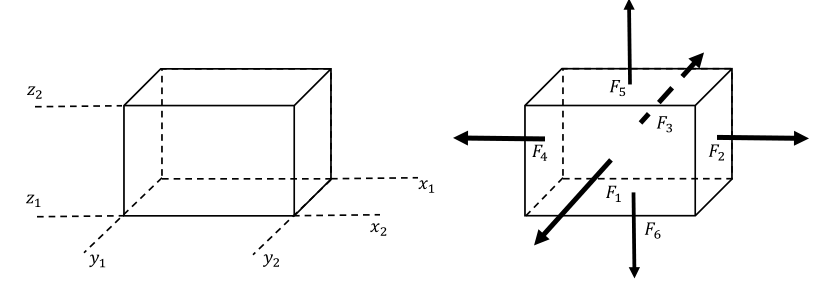
\includegraphics[scale=.5]{boxes}\end{center}
Realize that 
$$ \mathlarger\iiint_{R}\left( \frac{\p f}{\p x} + \frac{\p g}{\p y} + \frac{\p h}{\p z} \right)\,dx\,dy\,dz = \mathlarger\iiint_{R}  \frac{\p f}{\p x}\,dx\,dy\,dz  + \mathlarger\iiint_{R}  \frac{\p g}{\p y}\,dx\,dy\,dz + \mathlarger\iiint_{R} \frac{\p h}{\p z} \,dx\,dy\,dz.$$
Since it is given that $\iiint_{R}  \frac{\p f}{\p x}\,dx\,dy\,dz = \iint_{F_1} f\,dy\,dz + g\,dz\,dx + h\,dx\,dy +  \iint_{F_3} f\,dy\,dz + g\,dz\,dx + h\,dx\,dy$, I will compute $\iiint_{R}  \frac{\p g}{\p y}\,dx\,dy\,dz$ and $\iiint_{R} \frac{\p h}{\p z} \,dx\,dy\,dz.$ \\
First, I will use Fubini's Theorem to switch the order of integration. So,
$$ \mathlarger\iiint_{R}  \frac{\p g}{\p y}\,dx\,dy\,dz = \mathlarger\iiint_{R}  \frac{\p g}{\p y}\,dy\,dx\,dz$$
Now,
$$ \mathlarger\iiint_{R}  \frac{\p g}{\p y}\,dy\,dx\,dz = \mlvarint\limits_{z=z_1}^{z_2}\left[\mlvarint\limits_{x=x_1}^{x_2} g(x,y_2,z)\,dx\right]dz - \left(- \mlvarint\limits_{z=z_1}^{z_2}\left[\mlvarint\limits_{x=x_1}^{x_2} g(x,y_1,z)\,dx\right]dz\right)$$
The extra negative sign was picked up because really because the first integral on the last line is actually on $F_2$ and the second integral is on $F_4$. So, $F_4$ is oriented opposite $F_2$, so I needed to put an extra negative sign to account for that. So, now I have
$$\mathlarger\iiint_{R}  \frac{\p g}{\p y}\,dx\,dy\,dz = \mathlarger\iiint_{F_2}  g \,dy\,dx\,dz + \mathlarger\iiint_{F_4}  g \,dy\,dx\,dz$$
Using the fact that on $F_2$ and $F_4$, $dy = 0$ I can rewrite this as 
\begin{align*}& \quad \mathlarger\iiint_{R}  \frac{\p g}{\p y}\,dx\,dy\,dz = \bigiint{F_2}{}  g \,dx\,dz + \bigiint{F_4}{}  g\,dx\,dz\\
&= \bigiint{F_2}{} f \,dy\,dz + g \,dx\,dz + h\,dx\,dy + \bigiint{F_4}{} f \,dy\,dz + g \,dx\,dz + h\,dx\,dy.
\end{align*}
Moving onto calculating $\iiint_{R} \frac{\p h}{\p z} \,dx\,dy\,dz$, I will use Fubini's Theorem again to get
$$\iiint_{R} \frac{\p h}{\p z} \,dx\,dy\,dz = \iiint_{R} \frac{\p h}{\p z} \,dz\,dx\,dy.$$
Then,
$$ \mathlarger\iiint_{R}  \frac{\p h}{\p z}\,dz\,dx\,dy = \mlvarint\limits_{y=y_1}^{y_2}\left[\mlvarint\limits_{x=x_1}^{x_2} h(x,y,z_2)\,dx\right]dy - \left(- \mlvarint\limits_{y=y_1}^{y_2}\left[\mlvarint\limits_{x=x_1}^{x_2} h(x,y,z_1)\,dx\right]dy\right)$$
The extra negative sign was picked up because really because the first integral on the last line is actually on $F_5$ and the second integral is on $F_6$. So, $F_5$ is oriented opposite $F_6$, so I needed to put an extra negative sign to account for that. So, now I have
$$\mathlarger\iiint_{R}  \frac{\p g}{\p y}\,dx\,dy\,dz = \mathlarger\iiint_{F_5}  g \,dy\,dx\,dz + \mathlarger\iiint_{F_6}  g \,dy\,dx\,dz$$
Using the fact that on $F_5$ and $F_6$, $dz = 0$ I can rewrite this as 
\begin{align*}& \quad \mathlarger\iiint_{R}  \frac{\p h}{\p y}\,dx\,dy\,dz = \bigiint{F_5}{}  h \,dx\,dy + \bigiint{F_6}{}  h\,dx\,dy\\
&= \bigiint{F_5}{} f \,dy\,dz + g \,dx\,dz + h\,dx\,dy + \bigiint{F_6}{} f \,dy\,dz + g \,dx\,dz + h\,dx\,dy.
\end{align*}
Since
$$\mathlarger\iiint_{R}\left( \frac{\p f}{\p x} + \frac{\p g}{\p y} + \frac{\p h}{\p z} \right)\,dx\,dy\,dz = \mathlarger\iiint_{R}  \frac{\p f}{\p x}\,dx\,dy\,dz  + \mathlarger\iiint_{R}  \frac{\p g}{\p y}\,dx\,dy\,dz + \mathlarger\iiint_{R} \frac{\p h}{\p z} \,dx\,dy\,dz$$
by substitution I get that
\begin{align*}\mathlarger\iiint_{R}\left( \frac{\p f}{\p x} + \frac{\p g}{\p y} + \frac{\p h}{\p z} \right)\,dx\,dy\,dz &=   \bigiint{F_1}{} f\,dy\,dz + g\,dz\,dx + h\,dx\,dy +  \bigiint{F_3}{} f\,dy\,dz + g\,dz\,dx + h\,dx\,dy \\
&+\bigiint{F_2}{} f \,dy\,dz + g \,dx\,dz + h\,dx\,dy + \bigiint{F_4}{} f \,dy\,dz + g \,dx\,dz + h\,dx\,dy \\
&+ \bigiint{F_5}{} f \,dy\,dz + g \,dx\,dz + h\,dx\,dy + \bigiint{F_6}{} f \,dy\,dz + g \,dx\,dz + h\,dx\,dy
\end{align*}
Which is equivalent to
$$\bigiint{\p R}{} f \,dy\,dz + g \,dx\,dz + h\,dx\,dy$$
Therefore,
$$ \mathlarger\iiint_{R}\left( \frac{\p f}{\p x} + \frac{\p g}{\p y} + \frac{\p h}{\p z} \right)\,dx\,dy\,dz = \bigiint{\p R}{} f \,dy\,dz + g \,dx\,dz + h\,dx\,dy $$
\end{proof}

\begin{cproblem}{4}{White}\ \\
\vspace{-1em}
\begin{center} 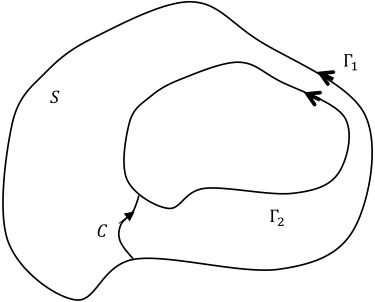
\includegraphics[scale=.40]{coolerblob}\end{center}
Prove that if $f(x,y), \ g(x,y)$ have continuous partial derivatives on $S\cup \p S$, then 
$$\bigiint{S}{} \left( \frac{\p g}{\p x} - \frac{\p f}{\p y} \right)dx\,dy = \mathlarger\oint_{\Gamma_1}f\,dx + g\,dy - \mathlarger\oint_{\Gamma_2}f\,dx + g\,dy.$$
\end{cproblem}
\begin{proof}
Imagine taking an infinitesimally small knife and cutting straight through $S$ from $\Gamma_1$ to $\Gamma_2$. This creates a new curve $C$ connecting $\Gamma_1$ and $\Gamma_2$. This new path can be defined as $\p S\setminus C = \Gamma_1 \cup C \cup -\Gamma_2 \cup -C$. This is because you can imagine traveling counterclockwise from $\Gamma_1$ across $C$ and then around $\Gamma_2$ clockwise $(-\Gamma_2)$ and back out to $\Gamma_1$ via $-C$ for connection. In creating this path we create and edge around a new surface called $S\setminus C$. Now, this line integral of my new path can be described as 
$$\boint{\Gamma_1}{} f\,dx + g\,dy + \boint{C}{}  f\,dx + g\,dy - \boint{\Gamma_2}{}f\,dx + g\,dy - \boint{-C}{}f\,dx + g\,dy = \boint{\p S\setminus C}{}f\,dx + g\,dy.$$
Now, applying Green's Theorem to this I get,
$$\boint{\p S\setminus C}{}f\,dx + g\,dy  = \bigiint{S\setminus C}{} \left( \frac{\p g}{\p x} - \frac{\p f}{\p y} \right)dx\,dy.$$
Notice that 
$$\bigiint{S\setminus C}{} \left( \frac{\p g}{\p x} - \frac{\p f}{\p y} \right)dx\,dy = \bigiint{S}{} \left( \frac{\p g}{\p x} - \frac{\p f}{\p y} \right)dx\,dy - \bigiint{C}{} \left( \frac{\p g}{\p x} - \frac{\p f}{\p y} \right)dx\,dy$$
and the integral over a curve is always zero because curves have zero area. So this becomes
$$ \bigiint{S\setminus C}{} \left( \frac{\p g}{\p x} - \frac{\p f}{\p y} \right)dx\,dy = \bigiint{S}{} \left( \frac{\p g}{\p x} - \frac{\p f}{\p y} \right)dx\,dy$$
Now by substiution it must be true that,
$$ \boint{\p S\setminus C}{}f\,dx + g\,dy  = \bigiint{S\setminus C}{} \left( \frac{\p g}{\p x} - \frac{\p f}{\p y} \right)dx\,dy =  \bigiint{S}{} \left( \frac{\p g}{\p x} - \frac{\p f}{\p y} \right)dx\,dy.$$
and it is easy to see that in the definition of $\oint_{\p S\setminus C}f\,dx + g\,dy$ that terms cancel out. Specifically, 
$$\boint{\p S\setminus C}{}f\,dx + g\,dy = \boint{\Gamma_1}{} f\,dx + g\,dy  - \boint{\Gamma_2}{}f\,dx + g\,dy + \boint{C}{}  f\,dx + g\,dy - \boint{-C}{}f\,dx + g\,dy =\boint{\Gamma_1}{} f\,dx + g\,dy  - \boint{\Gamma_2}{}f\,dx + g\,dy.$$
So, finally by substiution, it must be true that 
$$\boint{\p S\setminus C}{}f\,dx + g\,dy = \boint{\Gamma_1}{} f\,dx + g\,dy  - \boint{\Gamma_2}{}f\,dx + g\,dy  = \bigiint{S\setminus C}{} \left( \frac{\p g}{\p x} - \frac{\p f}{\p y} \right)dx\,dy =  \bigiint{S}{} \left( \frac{\p g}{\p x} - \frac{\p f}{\p y} \right)dx\,dy $$
This proves that when $f(x,y), \ g(x,y)$ have continuous partial derivatives on $S\cup \p S$, then
$$\bigiint{S}{} \left( \frac{\p g}{\p x} - \frac{\p f}{\p y} \right)dx\,dy = \mathlarger\oint_{\Gamma_1}f\,dx + g\,dy - \mathlarger\oint_{\Gamma_2}f\,dx + g\,dy.$$
\end{proof}

\begin{cproblem}{5}{White}
Recall that by Coulomb's Law, the electric field $\vec{E}$ generated by a point charge $q$ at the origin is given by
$$ \vec{E} = \frac{q}{4\pi\epsilon_0} \frac{\vec{r}}{r^3} = \frac{q}{4\pi\epsilon_0}\frac{1}{\left(x^2 + y^2 + z^2\right)^{\frac{3}{2}}}\bmat{x \\ y \\ z}$$
\begin{itemize}
\item[a.] Suppose $R$ is a closed, bounded region which does not contain the origin. Use the Divergence Theorem to show that the flux of $\vec{E}$ through $\p R$ is zero.
\item[b.] Suppose that the region $R$ contains the origin. Show that the flux of $\vec{E}$ through $\p R$ is given by $\frac{q}{\epsilon_0}$
\end{itemize}
\end{cproblem}
\begin{solution}
\begin{itemize}\vspace{-2em}
\item[a.] The flux through the region can be described as
$$ \bigiint{\p R}{}E_1\,dy\,dz + E_2\,dz\,dx + E_3\,dx\,dy $$
as similarly described in problem 2. Now, applying the Divergence Theorem on this I get
$$\bigiint{\p R}{}E_1\,dy\,dz + E_2\,dz\,dx + E_3\,dx\,dy  = \mathlarger\iiint_{R} \frac{\p E_1}{\p x} + \frac{\p E_2}{\p y} + \frac{\p E_3}{\p z}\,dx\,dy\,dz$$
I also derive through quotient rule that
\begin{align*}
\frac{\p E_1}{\p x} &= \frac{(x^2 + y^2 + z^2)^{\frac{3}{2}} - 3x^2\sqrt{(x^2 + y^2 + z^2)} }{(x^2 + y^2 + z^2)^3} = \frac{r^3 - 3x^2r}{r^6} = \frac{r^2 -3x^2}{r^5}\\
\frac{\p E_2}{\p x} &= \frac{(x^2 + y^2 + z^2)^{\frac{3}{2}} - 3y^2\sqrt{(x^2 + y^2 + z^2)} }{(x^2 + y^2 + z^2)^3} = \frac{r^3 - 3y^2r}{r^6} = \frac{r^2 -3y^2}{r^5} \\
\frac{\p E_3}{\p x} &= \frac{(x^2 + y^2 + z^2)^{\frac{3}{2}} - 3z^2\sqrt{(x^2 + y^2 + z^2)} }{(x^2 + y^2 + z^2)^3} = \frac{r^3 - 3z^2r}{r^6} = \frac{r^2 -3z^2}{r^5}
\end{align*}
and by substitution,
$$\bigiint{\p R}{}E_1\,dy\,dz + E_2\,dz\,dx + E_3\,dx\,dy =  \mathlarger\iiint_{R} \frac{\p E_1}{\p x} + \frac{\p E_2}{\p y} + \frac{\p E_3}{\p z}\,dx\,dy\,dz = \mathlarger\iiint_{R} \frac{r^2 -3x^2}{r^5} + \frac{r^2 -3y^2}{r^5} + \frac{r^2 -3z^2}{r^5}\,dx\,dy\,dz $$
which simplifies to
$$\mathlarger\iiint_{R} \frac{3r^2 - 3(x^2 + y^2 + z^2)}{r^5} \,dx\,dy\,dz = \mathlarger\iiint_{R} \frac{3r^2 - 3r^2}{r^5} \,dx\,dy\,dz = \mathlarger\iiint_{R} 0 \,dx\,dy\,dz = 0.$$
Therefore the total flux of $\vec{E}$ through $\p R$ is zero.
\item[b.] Imagine a  sphere $S$ with radius $a$ small enough such that $S \subset R$. Then, from the result of part a and the Divergence Theorem I know that the flux through $\p R$ is equal to the flux through $\p S$. So, I know that from a previous problem that flux of $\vec{A}$ on a sphere is described by
$$ \bigiint{S}{} A_1 \frac{\p (y,z)}{\p (\phi, \theta)} + A_2 \frac{\p (z,x)}{\p (\phi, \theta)} + A_3 \frac{\p (x,y)}{\p (\phi, \theta)} d\phi\,d\theta.$$
When $\vec{A} = \vec{E}$, I get that the flux is described as 
$$\frac{q}{4\pi\epsilon_0} \bigiint{S}{} \frac{x}{\left(x^2 + y^2 + z^2\right)^{\frac{3}{2}}}\frac{\p (y,z)}{\p (\phi, \theta)} + \frac{y}{\left(x^2 + y^2 + z^2\right)^{\frac{3}{2}}} \frac{\p (z,x)}{\p (\phi, \theta)} + \frac{z}{\left(x^2 + y^2 + z^2\right)^{\frac{3}{2}}} \frac{\p (x,y)}{\p (\phi, \theta)} d\phi\,d\theta.$$
where
\begin{align*}
x  &= a\sin(\phi)\cos(\theta) \\
y &= a\sin(\phi)\cos(\theta) \\ 
z &= a\cos(\phi)
\end{align*}
When these values are substituted I get that the total flux is $\frac{q}{\epsilon_0}$ on $\p S$. Since the flux on $\p S$ is equivalent to the flux on $\p R$, the flux through $\p R = \frac{q}{\epsilon_0}.$ 
\end{itemize}
\end{solution}
\end{document}